\documentclass[12pt]{article}

%\usepackage[T1]{fontenc}     % För svenska bokstäver
%\usepackage[swedish]{babel}  % För svensk avstavning och svenska

\usepackage{amsmath}
\usepackage{graphicx}
\usepackage{verbatim} 
\usepackage{color}
\usepackage{subfigure}
\usepackage{hyperref} 
\usepackage{listings}

\title{Project in FAFF25}
\author{Niklas Sundin Johansson, dt08njo\\Lars Gustafson, ada10lgu }

\begin{document}
\maketitle

\section{Projection Error}

\subsection{Implemation}

\subsection{Theroy}
Som Newton upptäckte så har olika våglängder av ljus olika brytningsindex i samma material, detta kallas kromatisk aberration. Fel kan uppstå även med monokromatisk ljus vid användandet av sfäriska prismor, detta kallas då sfärisk aberration. I uppgiften skall man med hjälp av, så kallad, ray tracing beräkna de fel som genereras. Genom att simulera standardstrålar och beräkna dess bana.  

Brytningslagen, $n_1 \cdot sin(\alpha _1) = n_2 \cdot sin(\alpha _2) $ används för att beräkna var fokalpunkten hamnar beroende på de två mediernas brytningsindex samt in och utfallsvinklarna vid övergången. 

Materialet BK7 används då kromatisk abberation skall beräknas. Formeln för dess brytningsindex är som nedan och gavs av uppgiften.\\
$n^2 = a_1 + a_2 \lambda^2 + a_3 \lambda^{-2}+a_4 \lambda^{-4}+a_5 \lambda^{-6}+a_6\lambda^{-8}$\\
$a_1= 2,271176$\\
$a_2 = -9.700709 \cdot 10^{-3}*\mu m^{-2}$\\
$a_3 = 0.0110971 \cdot \mu m^2$\\
$a_4 = 4.622809 \cdot 10^{-5} \cdot \mu m^4$\\
$a_5 = 1.616105 \cdot 10^{-5} \cdot \mu m^6$\\
$a_6 = -8.285043 \cdot 10^{-7} \cdot \mu m^8$

\subsection{Method}
Först beräknas felet, som en sfärisk prism genererar när man ökar höjden,$h$, från den optiska axeln. Detta jämnförs med 


\subsection{Result}

\subsubsection{A: Paraxial Approximation}
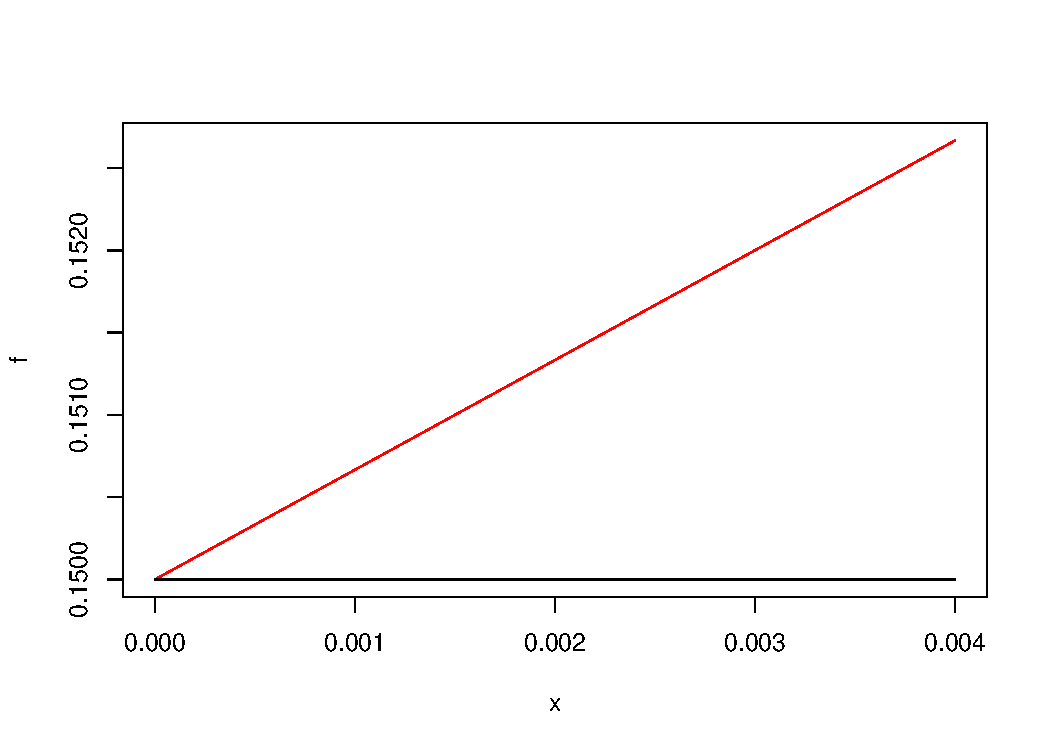
\includegraphics[scale=0.6]{para_approx.pdf}
With Paraxial Approximation focus point always becomes $0.15$ m, independent 
of where on the lins a beam parallel with the optic normal axis refract on the lens.
Mean while without the approximation it will drift futher away from the lins 
when the standard beam closes the edge of the lens.
$$write$$ $$down$$ $$difference$$ $$[placeholder]$$

\subsubsection{B: Material Replacement}
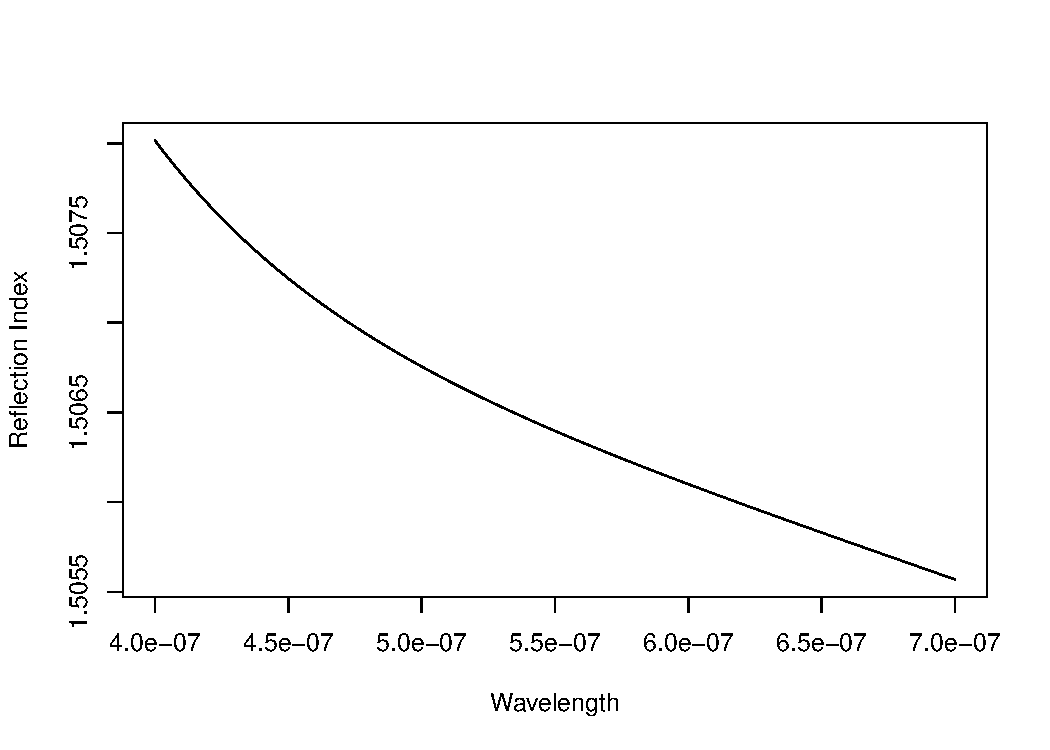
\includegraphics[scale=0.6]{BK7_index.pdf}
When plotting BK7 refraction index compared to wavelength of the incoming light,
the graph shows that $\Delta$ $0.0025$ in index between lowest value 
$400 nm$ and highest $700 nm$.
The function is close to liner at the high spectrum, which is wort noting.

\subsubsection{C: Chromatic Aborations}
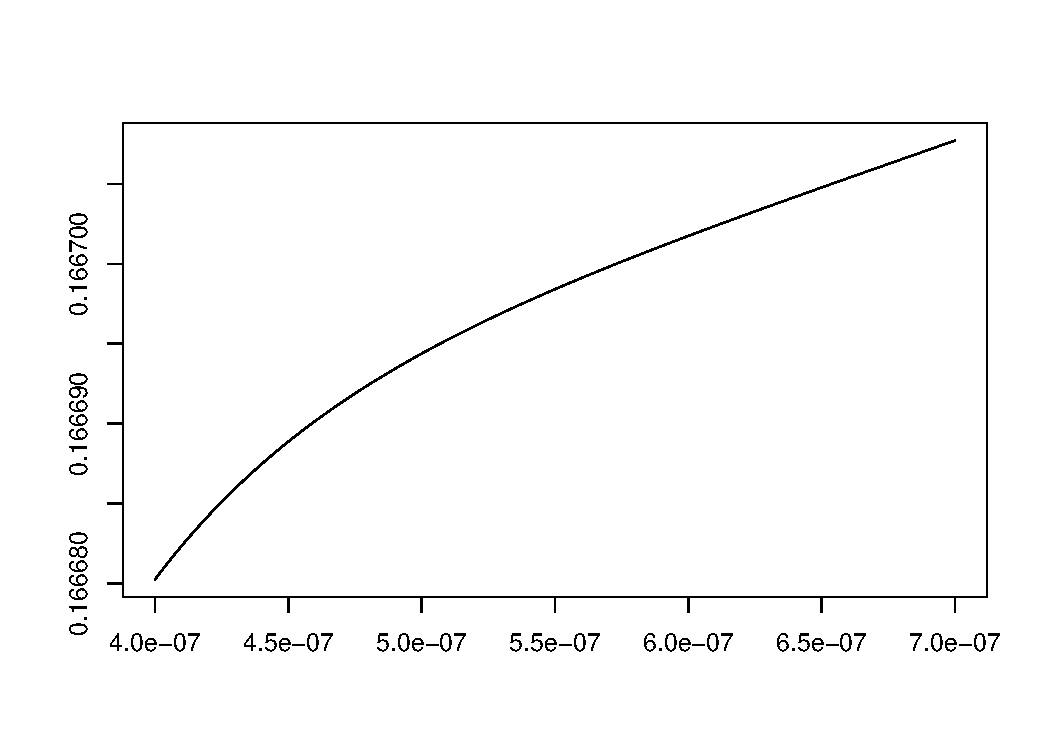
\includegraphics[scale=0.6]{BK7_abo.pdf}
Applying the BK7 material on the none Paraxial Approximated function, gives us
an $\Delta$ in focus point of close to $0.00028$. Generally close to $0.15$

\subsection{Conclusion and Commentary}
Replacement material $BK7$ has the properties to almost bring focus back to $0.15$, where it was when we applied Paraxial Approimation. 
Conclusion with the new material we can easy apply Paraxial Approximation
without to large errors in calculations, depending on specification limitation of cource. 

\subsection{Conclusion}

\section{Laser Pulse}

\subsection{Implemation}

\subsection{Result}
\subsubsection{A: Nummeric Solution}

\subsubsection{B: Differential Plot}
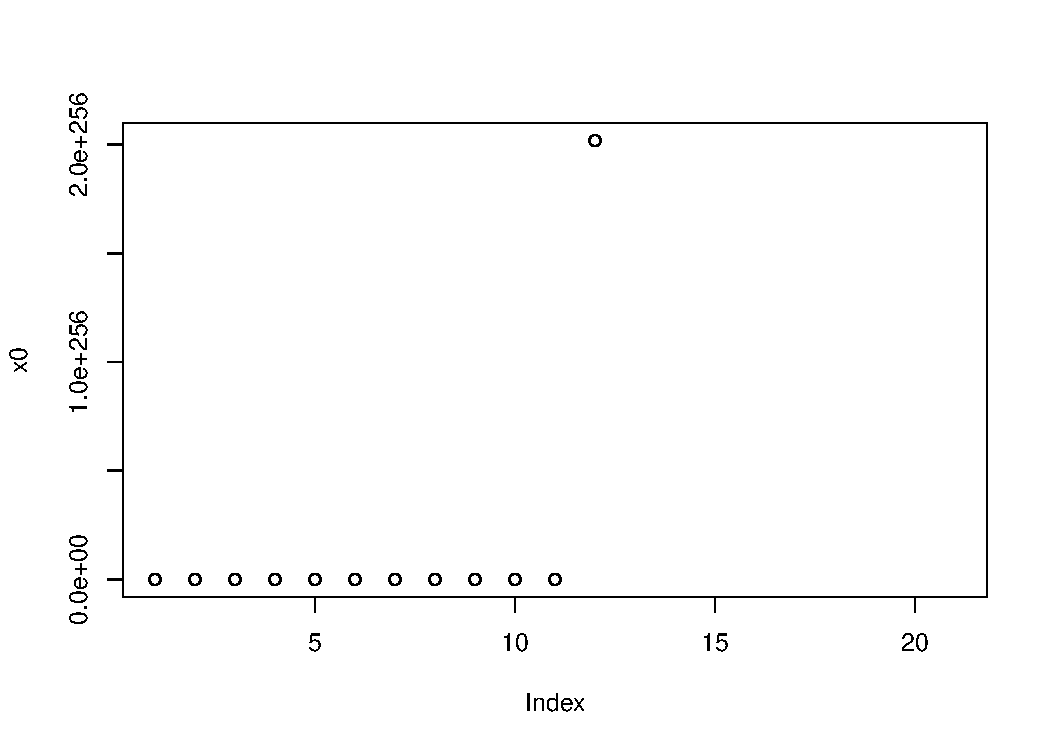
\includegraphics[scale=0.6]{N.pdf}

\subsection{Conclusion and Commentary}

\subsection{Conclusion}

\newpage
\appendix
\section{Implementation R Code}
\subsection{Assignment I:}
\lstinputlisting[numbers=left, keepspaces=true, firstline=0, lastline=68, language=R, basicstyle=\ttfamily\tiny]{datoruppgift.r}
\subsection{Assignment II: }
\lstinputlisting[numbers=left, keepspaces=true, firstline=68, basicstyle=\ttfamily\tiny]{datoruppgift.r}
\end{document}
